\chapter{Enhancement of Compound Selectivity Using a Radio Frequency Ion Funnel Proton Transfer Reaction Mass Spectrometer: Improved
Specificity for Explosive Compounds}
\markboth{Explosives in RFIF-PTR-ToF-MS}{}


This chapter is a reformatted copy of my published article (reference \cite{RF_TNT}):

\fullcite{RF_TNT}.


%Reprinted with permission from {COMPLETE REFERENCE CITATION}. Copyright {YEAR} American Chemical Society






\section*{Declaration of contribution}
My contribution to the article of which the present chapter is composed of was
in the discussion and writing process of the manuscript. 
%I repeated some of the measurements here presented, although the ones in the paper are those from Ram\'on Gonz\'alez-M\'endez.

\section{Abstract}
A key issue with any analytical system based on mass spectrometry with no initial separation of compounds is to have a high level of confidence in chemical assignment. This is particularly true for areas of security, such as airports, and recent terrorist attacks have highlighted the need for reliable analytical instrumentation. Proton transfer reaction mass spectrometry is a useful technology for these purposes because the chances of false positives are small owing to the use of a mass spectrometric analysis. However, the detection of an ion at a given \textit{m/z} for an explosive does not guarantee that that explosive is present. There is still some ambiguity associated with any chemical assignment owing to the presence of isobaric compounds and, depending on mass resolution, ions with the same nominal \textit{m/z}. In this article we describe how for the first time the use of a radio frequency ion-funnel (RFIF) in the reaction region (drift tube) of a proton transfer reaction -- time-of-flight -- mass spectrometer (PTR-ToF-MS) can be used to enhance specificity by manipulating the ion-molecule chemistry through collisional induced processes. Results for trinitrotoluene, dinitrotoluenes, and nitrotoluenes are presented to demonstrate the advantages of this new RFIF-PTR-ToF-MS for analytical chemical purposes.

\textbf{\textit{Keywords}}: Ion-Funnel; PTR-MS; Explosives; proton transfer reactions; reduced electric field; collisional induced dissociation.





\section{Introduction}

Ion funnels (IF) have been used since the late 1990s in conjunction with several ionisation and mass spectrometric techniques with a key purpose of increasing ion transmission efficiency and hence instrumental sensitivity and dynamic range \cite{shaffer1997novel,kelly2010ion}. Of relevance to our study, Schaffer et al. developed a radio-frequency (RF) IF for focusing and transmitting ions from relatively high pressure (> 1 Torr) ion sources to mass spectrometers \cite{shaffer1997novel}. Given that the typical operating pressure of a drift tube used in proton transfer reaction mass spectrometry (PTR- MS) is close to the optimum pressure for the operation of a RFIF, Kore Technology Ltd. designed and developed a RFIF to be incorporated into drift tubes in order to increase the instruments sensitivity \cite{barber2012increased}. This compact drift tube can simultaneously operate as an ion funnel and a reaction region with a controllable reaction time (dependent on the voltage supplied across the tube). The funnel design and the supplied RF and DC fields act in such a way to channel reagent and product ions towards the exit orifice of the drift tube so that more ions leave the reaction region into the much lower pressure mass spectrometric region, thereby decreasing the loss of ions that occurs at the end of the drift tube. The proof-of principle study reported increases in sensitivity of this RFIF-PTR-ToF-MS system that were found to be dependent on the \textit{m/z} of the product ions, but were typically between 1 and 2 orders of magnitude. For example enhancement factors of 45 and 200 were reported for protonated acetaldehyde and protonated acetone, respectively, at a reduced electric field of 120 Td (where this field refers to the DC voltage applied across the drift tube) \cite{barber2012increased}. 

Given that the RFIF forms part of the drift tube, we asked the question whether the high RF fields involved in the operation of an IF could be used to enhance collisions of the reagent and product ions with the buffer gas in the DT and hence change either the nature of the initial chemical ionisation process or induce collisional induced dissociation, respectively, occuring within the DT? We hypothesised that changes would result from raising the internal energy of the product ions and the energy of the reactions between reagent ions and neutral species through collisional processes as a result of the applied RF field. The real question is whether the RF collisional induced dissociation would lead to substantial fragmentation, or be more selective resulting in unique product ions that can be used to identify a chemical compound of interest with a higher specificity than that achievable just by using a standard drift tube at a given reduced electric field. Here we report details on a collaborative project involving KORE Technology Ltd. and the University of Birmingham which investigated the application of a RFIF drift tube of a PTR-ToF-MS for improved selectivity using several explosives as illustrative compounds, namely 2,4,6-trinitrotoluene (TNT), 2,4-, 2,6- and 3,4- dinitrotoluene (DNT) and 2-, 3- and 4-nitrotoluene (NT). We will show how the application of a RFIF leads to a higher confidence in compound identification. We thus demonstrate for the first time that the addition of a RFIF to a PTR-ToF-MS results in a more multi- dimensional analytical instrument that improves the selectivity that can be achieved by operating a drift tube of a PTR-MS in DC mode only.





\section{Methodology}

\subsection{Experimental details}

A KORE Technology Ltd. RFIF Series I PTR-ToF-MS was used. Details of KORE’s PTR- ToF-MS system with no IF has been described in detail elsewhere \cite{blake2004demonstration,ENNIS200572,RN445}, and hence only the salient points of this instrument are provided here. Using a needle valve, water vapour is introduced into a hollow cathode discharge where, after ionisation via electron impact and subsequent ion-molecule processes, the terminal reagent ion is H$_3$O$^+$ \cite{ellis2013proton}. These ions are transferred from the ion source into the drift tube (the reaction region) of the PTR-ToF-MS, which is typically at a pressure of 1 mbar and temperature 100 ºC, where they encounter the analyte. H$_3$O$^+$ ions react with the analyte M by donating their protons at the collisional rate, providing M has a proton affinity greater than that of water (PA(H$_2$O) = 691 kJ mol$^{-1}$). This process can be non-dissociative (resulting in the protonated molecule MH$^+$) and/or dissociative. Dissociative proton transfer results in product ions which may be useful in the identification of a compound. Fragmentation may be spontaneous upon proton transfer or may require additional energy which is supplied through collisions with the buffer gas resulting during the migration of ions under the influence of the electric field, E. The ratio of E to the buffer gas number density, N, is an important parameter (known as reduced electric field) which determines the mean collisional energy of ions with the neutral buffer gas. Hence it is the parameter often referred to and changed for investigating product ion branching ratios \cite{brown2010proton,sulzer2012proton,doi:10.1002/jms.2993,kassebacher2013investigations,sulzer2013applications,agarwal2014sensitivity,acton2014headspace,lanza2015selective}.

The IF (schematically shown in \autoref{fig:dt_diagram}) consists of 29 stainless steel plates of 0.2 mm thickness, mounted on precision-machined ceramic rods at an even spacing of 3.2 mm per plate. Tabs on the electrodes permit a resistor chain on a ceramic strip to be connected in addition to two capacitor stacks which allow the RF to be applied to the second half of the reactor. The orifice diameters of the plates through the first half of the stack is 40 mm, as used in the standard drift tube reactor. In the second half of the drift tube the orifice diameter steadily decreases to 6 mm at the final plate before the exit orifice. Across the complete ion- funnel a DC voltage is applied driving ions axially. When just operating with this voltage we shall refer to the instrument as operating in DC-only mode. In addition to this, to the second part of the drift tube a RF field can applied. The resonant frequency of the system is $\sim$760 kHz and the amplitude selected for the majority of the studies (peak-to-peak) was 200 V, which is superimposed on the dc voltage gradient across the drift tube. 

The main purpose of the RF field is to focus ions radially by creating repulsive effective potentials at the edges of the electrodes. However, in addition to this intended purpose, the RF results in ions oscillating between electrodes as they drift down the reactor. This gives ions higher collisional energies than those in the first half of the drift tube. We shall refer to operating the instrument with the RF on as RF-mode. At the end of the drift tube is a 400 ?m orifice, through which ions enter the ion transfer region for ToF-MS.


The use of specifying a reduced electric field, \textit{E/N}, is an appropriate parameter to use in DC-only mode, because it is well defined. In RF-mode (ion funnel on) the presence of DC and RF electric fields complicates the situation, because the electric field strength varies with distance from the RF electrodes, so that specifying a reduced electric field is not appropriate. \citeauthor{barber2012increased}  simply adopted an empirical effective reduced electric field by finding operating conditions for the ion-funnel drift tube that matched the performance of the same drift tube when operated under DC-only mode \cite{barber2012increased}. However, given that it is uncertain what the effective reduced electric field means, in this paper we refer to the DC voltage (Vdrift) applied across the drift tube.

A thermal desorption unit (TDU) connected to the inlet of the drift tube was used to introduce the explosive samples, details of which have been given elsewhere \cite{RN445}. The TDU, connecting lines and drift tube were operated at a temperature of 150$^{\circ}$C. PTFE swabs (ThermoFisher Scientific) onto which known quantities of explosives were deposited were placed into the TDU. The swabs came prepared from the manufacturer mounted on rectangular cardboard for easy insertion into the TDU. Once a seal was created, a carrier gas (in this study laboratory air) is heated to the temperature of the TDU before it flows through a series of holes in a heated metal plate. This heated air then passes through the swab and into the inlet system driving any desorbed material through to the drift tube creating a temporal concentration “pulse” of typically between 10 – 20 seconds of an explosive in the drift tube \cite{RN445}. Each swab provided one measurement, which was replicated three times and then the results were averaged and any background signals were subtracted. 

Explosive standards were purchased from AccuStandard Inc., New Haven, CT.
Typically these standards contained 0.1 mg of the explosive compound in 1 ml of solvent. For TNT, 2,4- and 2,6-DNT, and the NTs this involved an acetonitrile:methanol (1:1) mix. 3,4- DNT was just mixed with methanol. These samples were diluted in the appropriate solvent(s) (HPLC grade) to provide the required quantity of an explosive. Typically 1 µl of a solvent containing the required mass of an explosive was spotted onto a PTFE swab.















\subsection{Electronic structure calculations}
To aid in the interpretation of the experimental results a series of electronic structure calculations have been undertaken at 298 K. These involve density functional theory calculations using the GAUSSIAN09 PROGRAM with the GaussView 5 interface \cite{frisch2009gaussian}. The B3LYP functional with the 6-31+G(d,p) basis set was used throughout. Although it is appreciated that the drift tube temperature and the effective ion temperature are greater than 298 K, with the effective ion temperature being uncertain, the thermochemical calculations simply provide us with an indicator as to whether a reaction pathway is energetically possible or not.
















\section{Results and discussion}

\subsection{Reagent ions}
Before we begin discussing the results of the explosives, it is informative to present details on the reagent ion signal as a function of drift tube voltage, comparing intensities for DC-only mode (\autoref{fig:RF2}(a)) and RF-mode (funnel-on) (\autoref{fig:RF2}(b)) under identical operating conditions of hollow cathode and drift tube pressures and temperature. The observed decrease of H$_3$O$^+$ reagent ion signal with decreasing drift tube voltage is predominantly a result of the clustering with water molecules in the drift tube, which are not broken-up through collisions at lower drift tube voltages. The marked decrease in total reagent ion signal below about 50 Td is considered to be a result of the low SD potential, which scales with the DC drift tube potential. As the SD voltage decreases we can expect that fewer reagent ions reach the reactor entry.

\begin{figure}%[h]
\centering
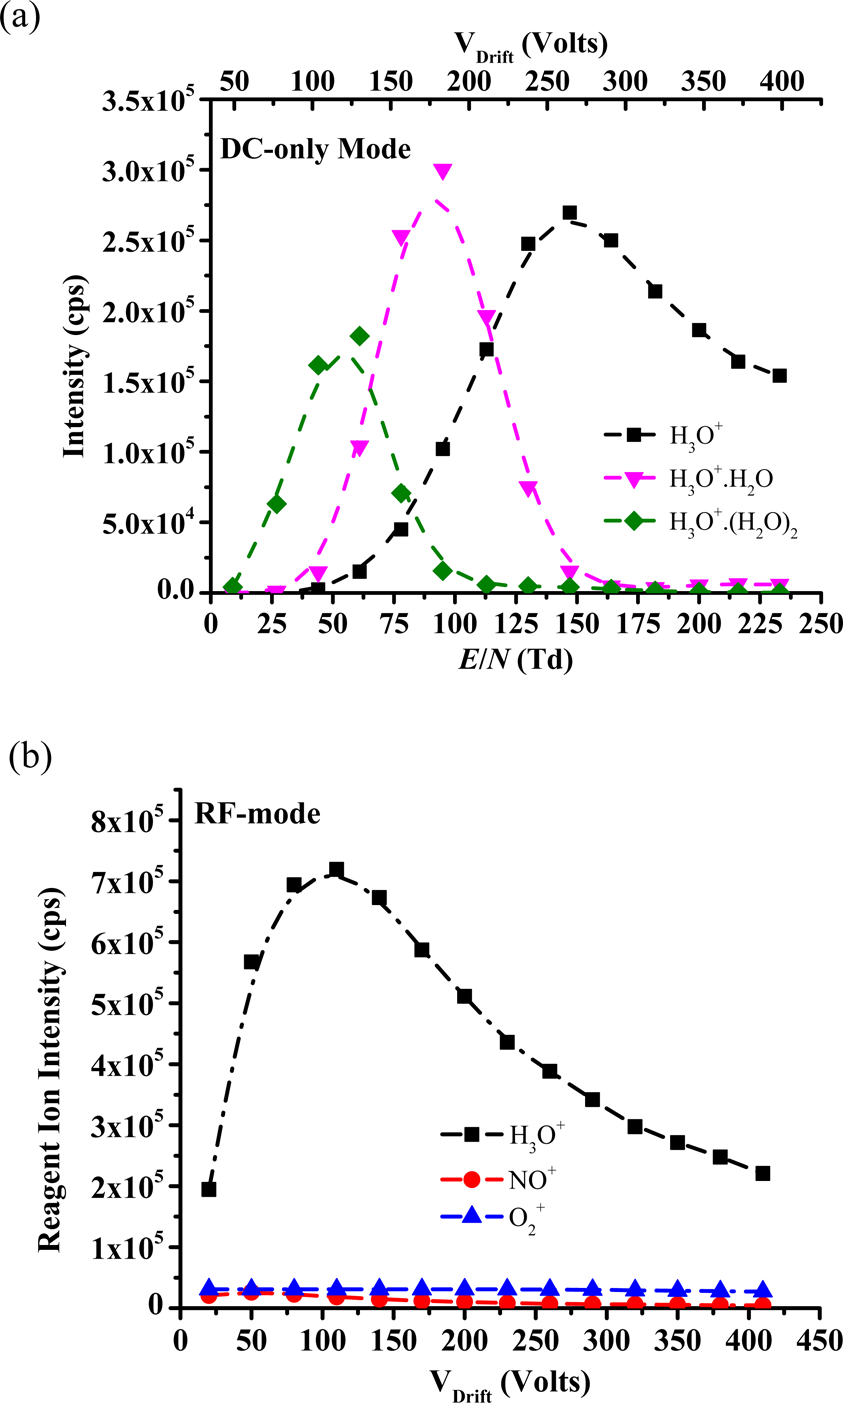
\includegraphics[height=0.7\textheight]{pics/RFpaper_fig2.png}
\caption{Ion intensities in counts per second (cps) of the water reagent ions present in the drift tube as a function of drift tube voltage (a) in DC-only mode and (b) in RF-mode (ion funnel on). For (b) the ion signals at \textit{m/z} 30 (NO$^+$) and 32 (O$_2^+$) are presented because
although low intensity they are still significant and are observed as a result of the improved ion transmission in RF-mode. In DC-mode the signal intensities of these ions are negligible and are therefore not presented.}
\label{fig:RF2}
\end{figure}

\autoref{fig:RF2}(a) shows that by 100 Td the H$_3$O$^+$ reagent ion signal has reduced significantly and that the protonated water clusters start to dominate at the lowest reduced electric field corresponding to a voltage drop across the drift tube of about 200 V under the operational temperature and pressure values used. (The actual percentage of protonated water clusters for fixed \textit{E/N} is also strongly dependent on the humidity of the buffer gas in the drift tube, which is dependent on the amount of forward flow of H$_2$O from the ion source into the drift tube and the humidity of the laboratory air.) In RF-mode no protonated water clusters are observed, because they are broken-up through collisions in the RFIF region of the drift tube. Furthermore, at about 120 V the H$_3$O$^+$ intensity is approximately at its maximum value. As the drift voltage decreases, the reagent ion signal decreases. However, even at a drift tube voltage of only 20 V (which in DC-only mode would correspond to a reduced electric field of only about 10 Td) there is still a significant reagent ion count. This enhancement of reagent ion signal at low drift tube voltages can only be a result of the trapping that the RF field provides thereby reducing the diffusional loss that occurs in DC-only mode under low drift tube voltages.













\subsection{This is mine -- Reagent ion in DC mode and RF mode}
As stated before, proton donation to the targeted analyte comes from the collisions with the reagent ions, so it is crucial to monitor their signal to know the amount of available protons to be transferred to the analyte.

The signal of the hydronium and its clusters as a function of the drift tube voltage in both DC mode and RF mode is shown in figure.......... 
These agree with the reagent ion signals previously observed \cite{price1977new}.
The $^{18}$O isotope peak is used to calculate the intensity of the reagent ions when their $^{16}$O peak is saturated. The natural composition of oxygen is $^{16}$O (99.76\%), $^{17}$O (0.03\%) and $^{18}$O (0.21\%) \cite{nistoxygen}. 

The reagent ions' dependence with the voltage in DC mode is very different to that in RF mode. In DC mode the clusters break apart as the drift voltage increases. On the other hand, the RF field in RF mode delivers an extra collisional energy that breaks the clusters apart independently of the drift voltage. Also, this RF field can create potential wells for the lighter masses generating a low-mass cut-off of the transmission \cite{Chung123}. It is also key to properly tune the capacitance from plate 29 to avoid ``closing'' the funnel.

The measured reagent ion signal depends on the clustering/declustering reactions and the transmission of the instrument. Furthermore, clustering depends on humidity, collisional energy (\textit{E/N}) and drift time. The higher the pressure in the cathode, the more hydronium is produced but it also will tend to create hydrogen bonds with other ions. Moreover, the higher the collisional energy, the more collisions the clusters will undergo, making them dissociate eventually. And last, the longer the drift time (at a given collisional energy), the more time the ions have to break apart through collisions.









\subsection{2,4,6-trinitrotoluene (TNT)}
Using both PTR-ToF-MS and PTR-Quad-MS systems Sulzer et al. have previously shown that there is an unusual dependence of the intensity of protonated TNT on the reduced electric field in that there is an increase in the sensitivity of detection with increasing \textit{E/N} \cite{sulzer2012proton,mayhew2010applications}. This increase continues until a maximum is reached at about 180 Td, after which the signal intensity shows the more usual behaviour of decreasing with increasing \textit{E/N}. This is opposite to what is commonly found in PTR-MS studies, because with reduced reaction times, fragmentation to non-specific product ions, and reduction in ion transmission the protonated molecule intensity reduces with increasing \textit{E/N}. The explanation of this unusual intensity dependence for TNTH$^+$ has been described in detail \cite{sulzer2012proton}. In brief, it is a result of a secondary reaction of TNTH$^+$.H$_2$O (which is readily formed at low \textit{E/N}) with H$_2$O leading to a terminal ion which does not contain TNT, namely H$_3$O$^+$.H$_2$O. 

In DC-only mode and when a product ion signal is detected, for all \textit{E/N} values investigated only one product ion is observed that contains the explosive, namely protonated TNT at \textit{m/z} 228. However, in RF mode, another fragment ion is found at \textit{m/z} 210, the intensity of which increases with decreasing drift tube voltage (i.e. decreasing \textit{E/N} in DC mode) down to values under which the PTR-ToF-MS does not perform in DC mode owing to a lack of sufficient transmission of ions to the mass spectrometer (\autoref{fig:RF2}(a)). Typical results obtained for TNT are shown in \autoref{fig:RF3}. That the fragment ion \textit{m/z} 210 intensity increases with decreasing drift tube voltage (\autoref{fig:RF3}) is perhaps not what is expected given that decreasing DC voltage means lower collisional energies. However, that only applies in the first half of the drift tube. As the drift tube voltage is reduced more collisions in the RFIF region of the drift tube occur, which in turn enhances collisional induced dissociation. Following proton transfer the protonated molecule gains sufficient internal energy
through collisions in the RFIF section of the drift tube to eliminate H$_2$O:
\begin{equation}
    H_3O^+ + TNT \rightarrow (TNTH^+)^* + H_2O
    \label{eq:rf1}
\end{equation}
\begin{equation}
     (TNTH^+)^* + M \rightarrow [TNT-H_2O]H^+ + H_2O + M
    \label{eq:rf2}
\end{equation}
where M is a buffer gas molecule. Thus specificity can be increased by either switching off and on the RFIF at a specific drift tube voltage or by switching the drift tube voltage. Note that a minor percentage of the observed \textit{m/z} 210 results from the reaction of the O$_2^+$ (always present in low concentrations in the drift tube as an impurity ion) with TNT via a dissociative charge transfer process leading to the loss of OH from TNT$^+$ \cite{sulzer2013applications}. 

\begin{figure}%[h]
\centering
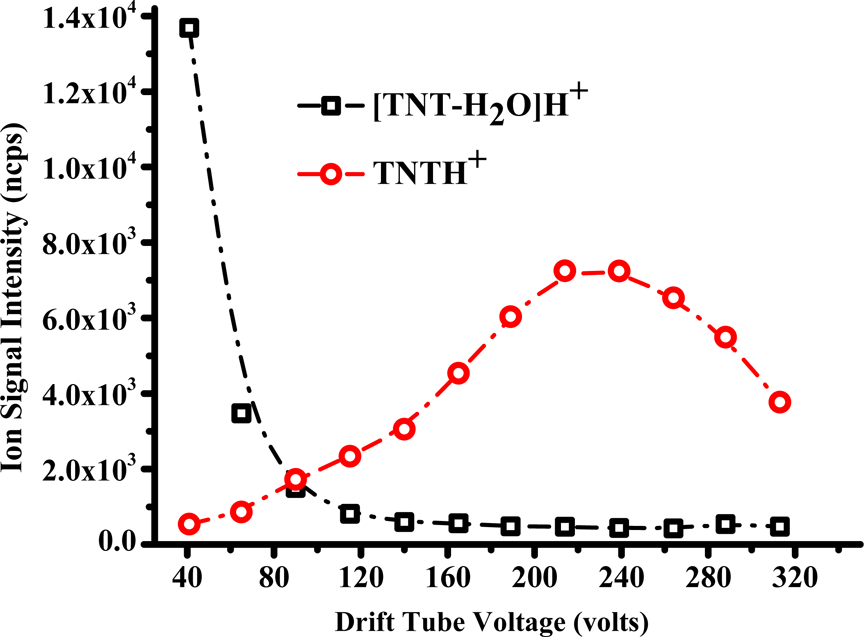
\includegraphics[height=0.3\textheight]{pics/RFpaper_fig3.png}
\caption{Product ion intensities as a function of drift tube voltage in RF mode. The data have been taken using 100 ng of TNT. The ion signals have been normalized to 10$^6$ H$_3$O$^+$ reagent ions and drift times. (The lines used in all graphs are just a guide to the eye.)}
\label{fig:RF3}
\end{figure}

That the reaction pathway leading to the elimination of H$_2$O is overall energetically favourable (\autoref{table:RF:tab1}) but is only observed in RF mode, is an indication that there must be an energy barrier for pathway (2). Evidence of this is provided from the results obtained when investigating the effects of changing the RF amplitude at fixed drift tube voltages and fixed frequency. \autoref{fig:RF4} provides a summary of these measurements, which shows that as the RF peak-to-peak voltage is decreased the intensity of the \textit{m/z} 210 decreases for all drift tube voltages.

\begin{figure}%[h]
\centering
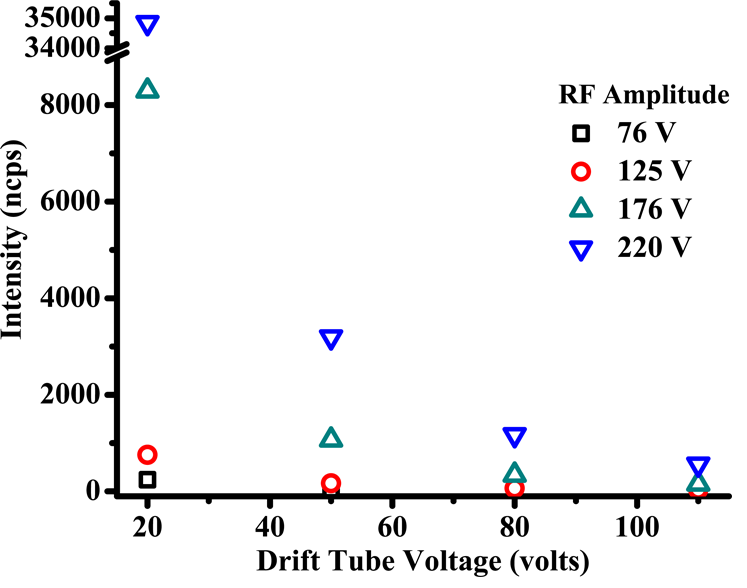
\includegraphics[height=0.3\textheight]{pics/RFpaper_fig4.png}
\caption{Intensities in ncps of the product ion [TNT - H$_2$O]H$^+$ as a function of drift tube voltage and RF amplitude (volts) with the frequency kept at 760 kHz (±3\%).
slightly}
\label{fig:RF4}
\end{figure}

\begin{table}%[]
\caption{Energetics for the proton transfer from H$_3$O$^+$ to TNT calculated using the B3LYP functional and the 6-31+G(d,p) basis set.}
\label{table:RF:tab1}
\begin{tabular}{lcc}
\hline
\textbf{Products} & \textbf{$\Delta$H$_{298}$ (kJ/mol)} & \textbf{$\Delta$G$_{298}$ (kJ/mol)} \\
\hline
TNTH$^+$(2NO$_2$syn) + H$_2$O  & -46   & -47     \\
TNTH$^+$(2NO$_2$anti) + H$_2$O & -55   & -55     \\
TNTH$^+$(4NO$_2$) + H$_2$O     & -68   & -60     \\
TS syn/anti + H$_2$O          & -9    & -5      \\ 
\hline
\end{tabular}
\end{table}

The initial step leading to \textit{m/z} 228 is the transfer of a proton from H$_3$O$^+$ to TNT. Protonation of TNT can occur on the nitro groups at the 2 and 4 positions, both having similar proton affinities, although as elimination of water from TNTH$^+$ will presumably involve the methyl group only protonation of the nitro group in the 2- position is of relevance. However, protonation on the 4 nitro will occur (the PA and GB are slightly greater than the 2 nitro) and this will reduce the amount of TNTH$^+$ available to lose water. Two configurations are
possible for protonation in the 2 position as illustrated in \autoref{fig:RF5}, with the anti being slightly more stable by ca. 8 kJ mol$^{-1}$. The transition state energetics for interconversion are $\Delta$H$_{298}$
 +46 kJ mol$^{-1}$ and $\Delta$G$_{298}$ +51 kJ mol$^{-1}$ above the anti conformation, but whichever is
formed there is sufficient energy in the initial protonation to allow rapid interconversion (\autoref{table:RF:tab1}).

\begin{figure}%[h]
\centering
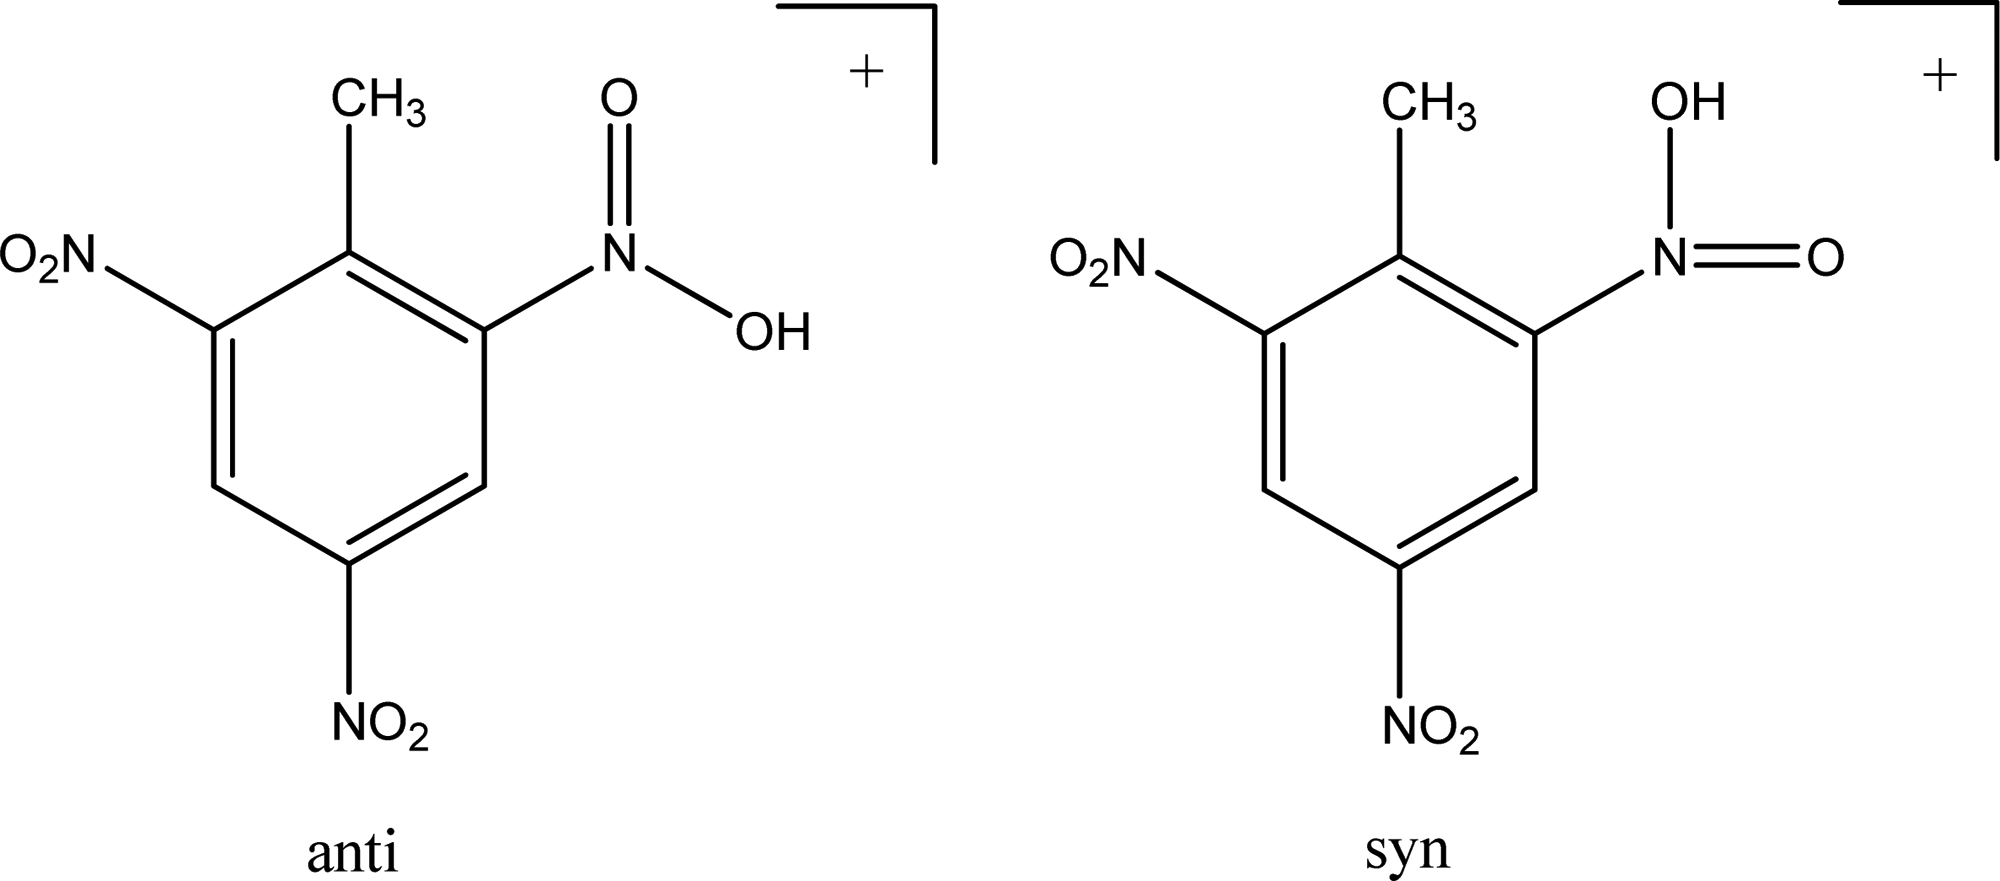
\includegraphics[height=0.2\textheight]{pics/RFpaper_fig5.png}
\caption{Two possible configurations resulting from protonation of TNT in the 2 position.}
\label{fig:RF5}
\end{figure}

There are three stable structures for the ion remaining after the elimination of water from TNTH$^+$ (\autoref{fig:RF6}). A fourth structure, similar to TNTH$^+$ - H$_2$O (b) with the hydrogens of the methylene group orthogonal to the ring, proved to be unstable and rearranged to TNTH$^+$ - H$_2$O (a) . The energetics for the transformation of TNTH$^+$ to TNTH$^+$ - H$_2$O (a-c) + H$_2$O are given in \autoref{table:RF:tab2}.


\begin{figure}%[h]
\centering
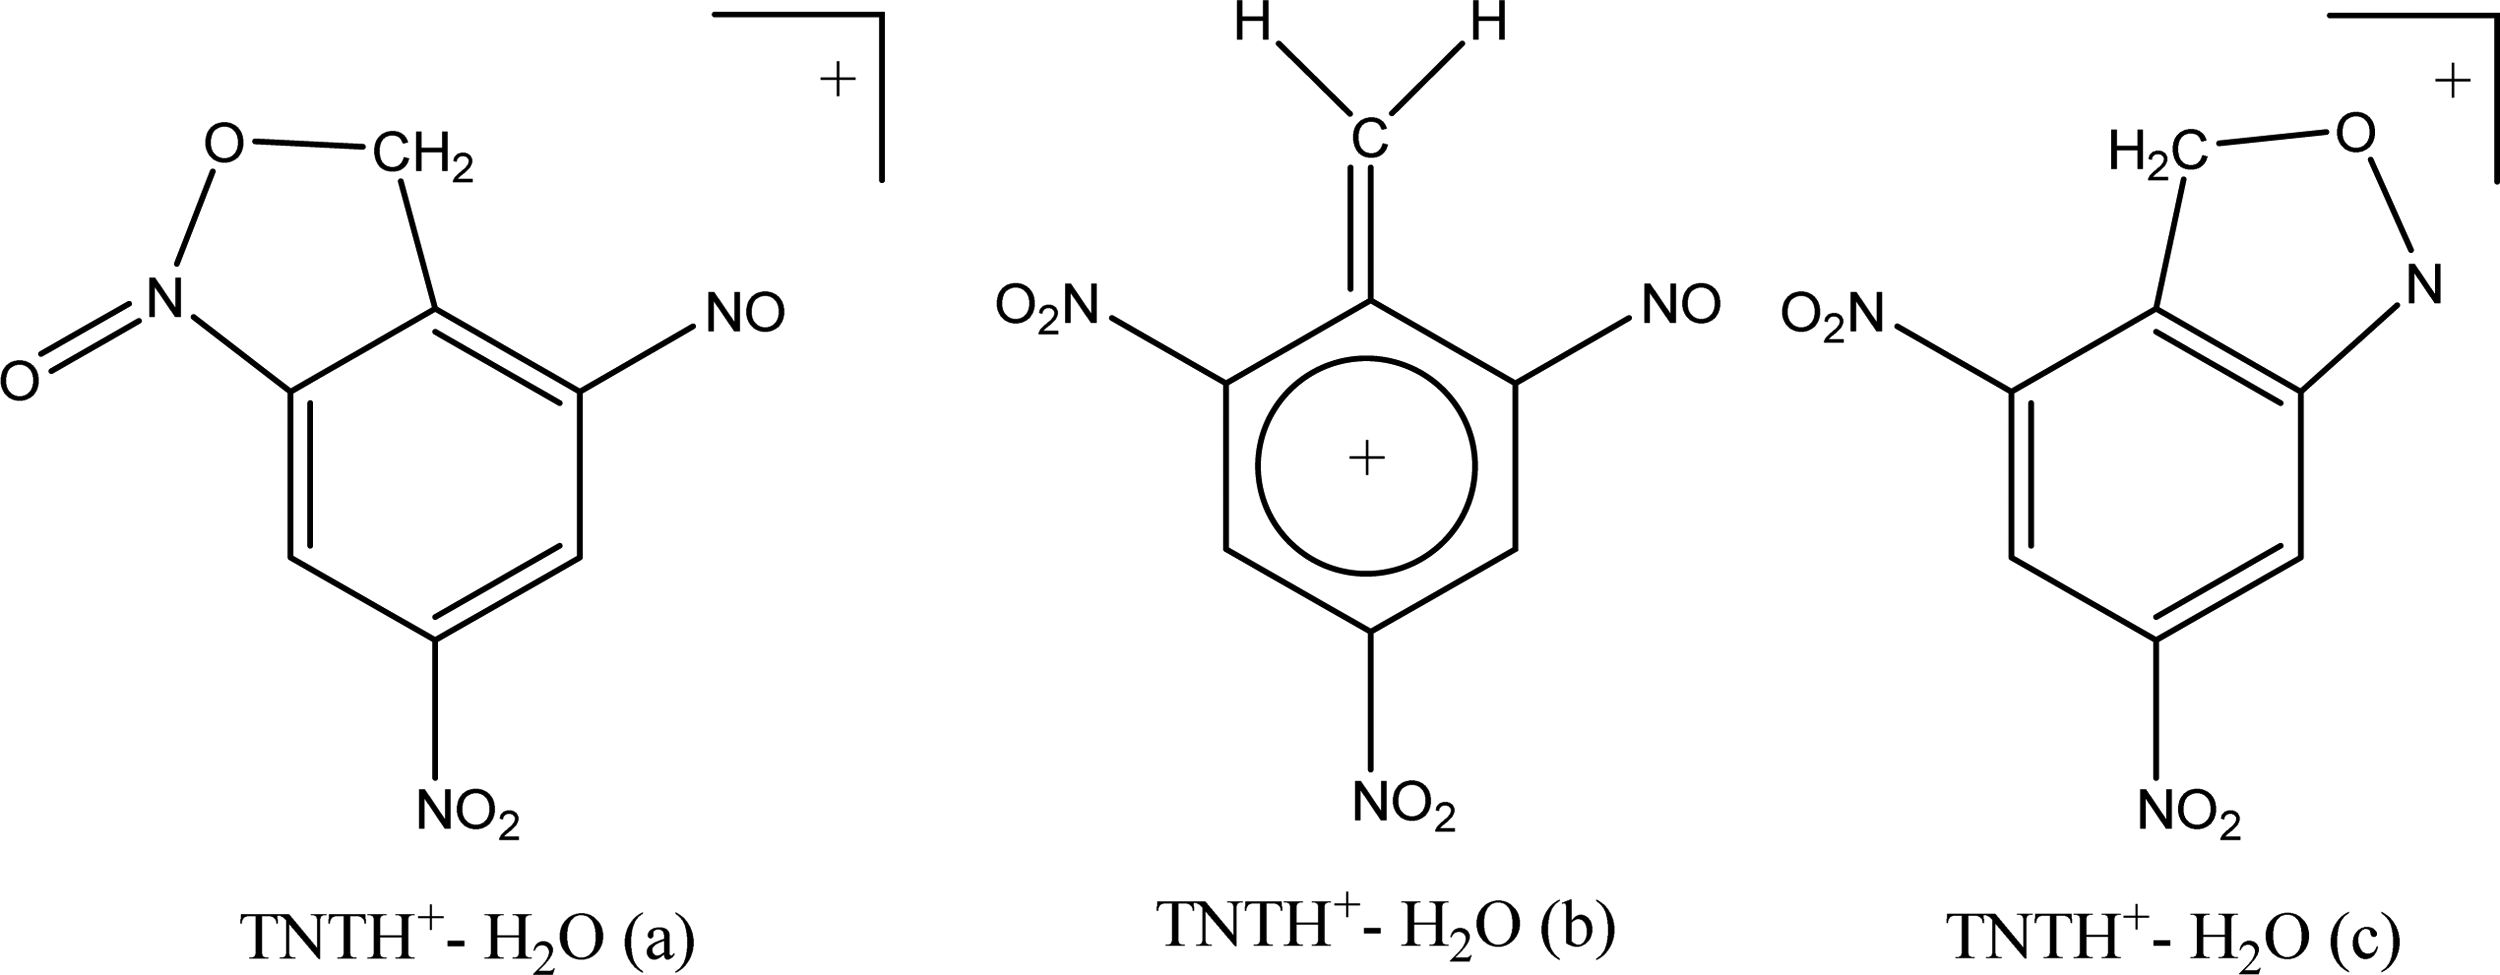
\includegraphics[height=0.2\textheight]{pics/RFpaper_fig6.png}
\caption{Stable structures of the [TNT - H$_2$O]H$^+$ ion.}
\label{fig:RF6}
\end{figure}


\begin{table}%[]
\caption{Energetics for the elimination of water from TNT following proton transfer from H$_3$O$^+$ for the three stable structures shown in \autoref{fig:RF6}.}
\label{table:RF:tab2}
\begin{tabular}{lcc}
\hline
\textbf{Products} & \textbf{$\Delta$H$_{298}$ (kJ/mol)} & \textbf{$\Delta$G$_{298}$ (kJ/mol)} \\
\hline
TNTH$^+$ - H$_2$O (a) + 2H$_2$O & -104      & -145     \\
TNTH$^+$ - H$_2$O (b) + 2H$_2$O & +47       & -7     \\
TNTH$^+$ - H$_2$O (c) + 2H$_2$O & -128      & -168     \\
\hline
\end{tabular}
\end{table}

Various attempts using the QST3 approach were made to find transition states for these possible reactions but all lead to TNTH$^+$ - H$_2$O (c), though interestingly the transition state had a close resemblance to TNTH$^+$- H$_2$O (b). The transition state was characterised by one imaginary frequency and the internal reaction coordinate leading to TNTH$^+$- H$_2$O (c) in the forward direction and TNTH$^+$ with the proton on the 2-nitro group in the syn conformation in the reverse direction. The activation energies relative to TNT + H$_3$O$^+$ are $\Delta$H$_{298}$ +158 kJ mol$^{-1}$ and $\Delta$G$_{298}$ +162 kJ mol$^{-1}$. 

The presumption that the elimination of water from protonated TNT can only occur when the methyl and nitro groups are adjacent to each other was readily tested by investigating isomers of DNT and NT. For those isomers that satisfy the condition of an adjacent nitro and methyl group, then [DNT-H$_2$O]H$^+$ and [NT-H$_2$O]H$^+$ fragment ions should be observed, otherwise not. Thus we predicted to observe elimination of water from the 2,6-DNT, 2,4-DNT and 2-NT but not from 3,4-DNT, 3-NT or 4-NT following proton transfer in RF mode.







\subsection{Dinitrotoluenes}
In both RF-mode and DC-only mode for 3,4-DNT the only primary product ion that is observed with any significant intensity for all drift tube voltages is the protonated molecule. That no \textit{m/z} 165 is observed, which would correspond to the elimination of water from the protonated molecule, is in agreement with our prediction, because neither nitro group are adjacent to the methyl group. With decreasing drift tube voltage the protonated 3,4-DNT clusters with H$_2$O, leading to a reduction in the DNTH$^+$ signal. Whilst this is particularly
significant in DC-only mode, with DNTH$^+$.(H$_2$O)n (n = 1, 2 and 3) ions becoming the dominant product ions by about 100 Td, some water clustering is still observed in RF-mode. For example at a drift tube voltage of 20 V the percentage branching ratios are approximately 70\%, 20\% and 10\% for DNTH$^+$, DNTH$^+$.H$_2$O, and DNTH$^+$.(H$_2$O)2, respectively. 

For the 2,4- and 2,6-DNT isomers, at low drift tube voltages in addition to an observed ion at \textit{m/z} 201 corresponding to the DNTH$^+$.H$_2$O in RF-mode a product ion is observed at \textit{m/z} 165, which is [DNT-H$_2$O]H$^+$. \autoref{fig:RF7} illustrates this for 2,6-DNT, which shows that the probability for the elimination of water increases with decreasing drift tube voltage (the results for 2,4-DNT in RF-mode are similar, although the production for [DNT-H$_2$O]H$^+$ is less by about 10\%). In DC-only mode, \textit{m/z} 165 is also observed for 2,6-DNT, but its intensity only becomes significant when a high drift tube voltage is applied leading to reduced electric fields above about 180 Td, and even then the percentage ion product distribution is only approximately 10\% (\autoref{fig:RF8}). However, this can explain the slight increase in the production of \textit{m/z} 165 in \autoref{fig:RF7} when the applied drift tube voltage is above about 275 V. With increasing drift tube voltage additional fragment ions are found at \textit{m/z} 136 and 91, corresponding to an elimination of HONO and 2NO2, respectively, from the protonated molecule. These two ions are also found with significant intensities for 2,6-DNT when operating in DC-only mode when the reduced electric fields is greater than about 160 Td. That DNTH$^+$.H$_2$O is observed in RF mode at low drift tube voltages, when no protonated water clusters are observed (\autoref{fig:RF2} (b)), requires some explanation. We propose that following a collision the energy involved is distributed in more degrees of freedom for DNTH$^+$.H$_2$O than for H$_3$O$^+$.(H$_2$O)n and hence it is less likely for energy to be concentrated into losing the water molecule.

\begin{figure}%[h]
\centering
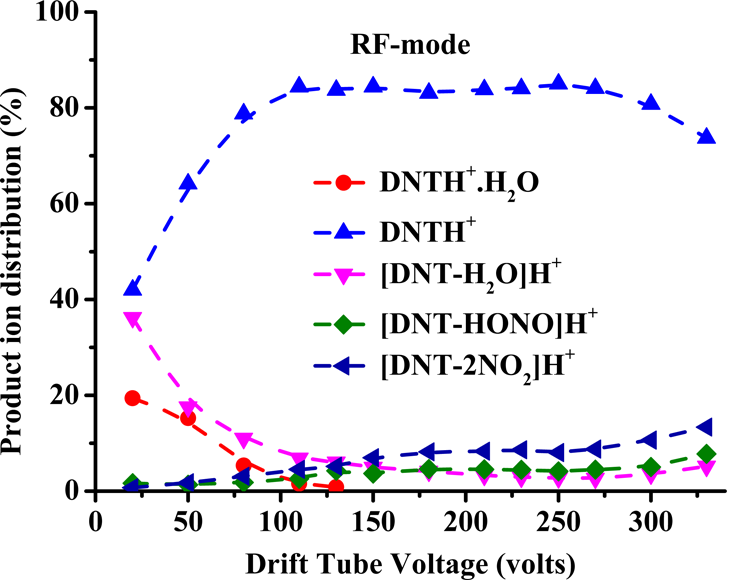
\includegraphics[height=0.3\textheight]{pics/RFpaper_fig7.png}
\caption{Percentage product ion distributions resulting from the reaction of H$_3$O$^+$ with 2,6-DNT in RF-mode including the secondary process resulting in the association of the protonated molecule with water as a function of supplied drift tube voltage.}
\label{fig:RF7}
\end{figure}

\begin{figure}%[h]
\centering
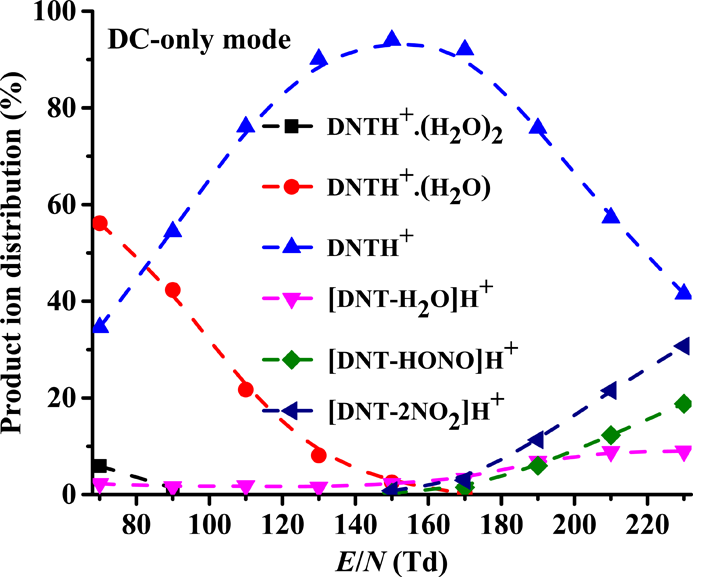
\includegraphics[height=0.3\textheight]{pics/RFpaper_fig8.png}
\caption{Percentage product ion distributions resulting from the reaction of H$_3$O$^+$ with 2,6-DNT in DC-only mode including the secondary process resulting in the association of the protonated molecule with water as a function reduced electric field.}
\label{fig:RF8}
\end{figure}

Building on the comprehensive investigation of the TNT system we can go straight to the salient structures and energetics for the loss of water from 2,4-DNT and 2,6-DNT following proton transfer from H$_3$O$^+$. These calculations are given in \autoref{table:RF:tab3} (a) and (b), respectively.

\begin{table}%[]
\caption{Energetics for the elimination of water from (a) 2,4-DNT and (b) 2,6-DNT following proton transfer from H$_3$O$^+$.}
\label{table:RF:tab3}
\begin{tabular}{lcc}
\hline
\multicolumn{3}{c}{(a)}\\
\hline
\textbf{Products} & \textbf{$\Delta$H$_{298}$ (kJ/mol)} & \textbf{$\Delta$G$_{298}$ (kJ/mol)} \\
\hline
2,4-DNTH$^+$(syn) + H$_2$O        & -89  & -87  \\
2,4-DNTH$^+$(anti) + H$_2$O       & -96  & -95  \\
TS syn/anti + H$_2$O           & -21  & -16  \\
TS for loss of H$_2$O + H$_2$O & +126 & +130 \\
2,4-DNT-H$_2$O (c) + 2H$_2$O   & -146 & -187 \\
\hline
\multicolumn{3}{c}{(b)}\\
\hline
\textbf{Products} & \textbf{$\Delta$H$_{298}$ (kJ/mol)} & \textbf{$\Delta$G$_{298}$ (kJ/mol)} \\
\hline
2,6-DNTH$^+$(syn) + H$_2$O        & -87  & -88  \\
2,6-DNTH$^+$(anti) + H$_2$O       & -95  & -95  \\
TS syn/anti + H$_2$O           & -42  & -38  \\
TS for loss of H$_2$O + H$_2$O & +117 & +120 \\
2,6-DNT-H$_2$O (c) + 2H$_2$O   & -177 & -217 \\
\hline
\end{tabular}
\end{table}

\subsection{Nitrotoluenes}
In order to further investigate the requirement of methyl and nitro functional groups to be adjacent in order to facilitate the elimination of water when using the RFIF, the three isomers of nitrotoluene have been investigated. We can expect in RF-mode that only 2-NT should have a reaction pathway which would lead to the elimination of water following proton transfer from H$_3$O$^+$. For 3-NT and 4-NT no such elimination should occur. A review of the resulting mass spectra for all three isomers shows that that is the case. However, the nitrotoluenes are more complicated than TNT and the DNTs, because other product ions are observed even at the lowest drift tube voltage. The NT isomers show significant fragmentation following proton transfer. This is found to occur in not only RF-mode but also DC-only mode. In addition to the elimination of water, which is not the dominant product ion, channels corresponding to the elimination of C2H4, NO, CH3NO, NO2 and HONO are observed in both modes. This is illustrated in \autoref{fig:RF9} for 2-NT when operating (a) in RF- mode and (b) in DC-only mode. At low drift tube voltages NTH$^+$.H$_2$O is observed (\autoref{fig:RF9}(a)) in RF mode, presumably for reasons described above for DNT.

\begin{figure}%[h]
\centering
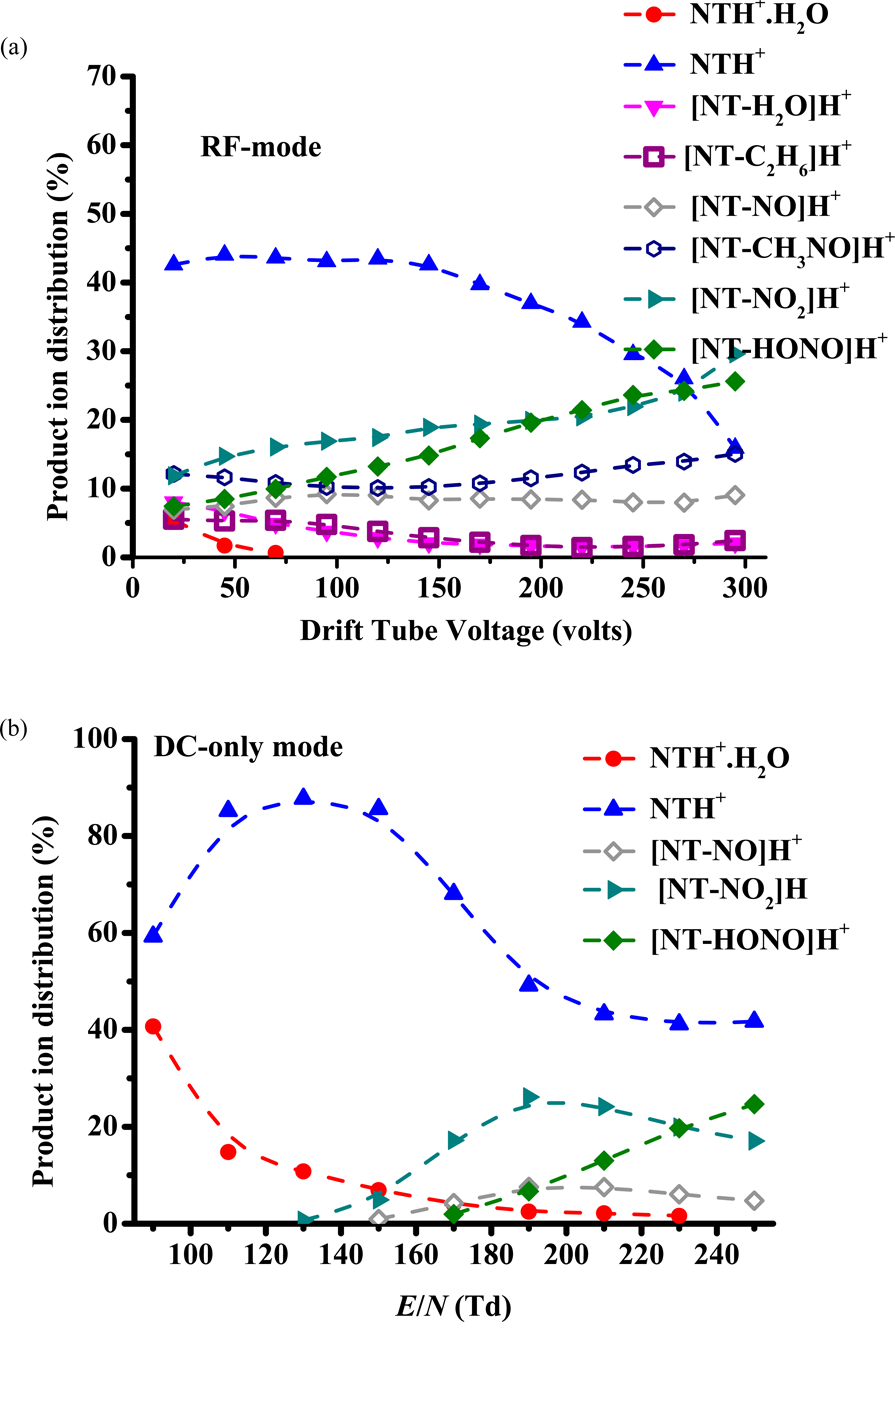
\includegraphics[height=0.7\textheight]{pics/RFpaper_fig9.png}
\caption{Percentage product ion distributions resulting from the reaction of H$_3$O$^+$ with 2-NT in (a) RF-mode and (b) DC-only mode as a function drift tube voltage. Included are the secondary ion-molecule processes resulting in the association of the protonated molecule with water.}
\label{fig:RF9}
\end{figure}

\autoref{table:RF:tab4} presents the DFT energetics calculations for the elimination of water for 2-NT following proton transfer from H$_3$O$^+$.


\begin{table}%[]
\caption{Energetics for the elimination of water from 2-NT following proton transfer from H$_3$O$^+$.}
\label{table:RF:tab4}
\begin{tabular}{lcc}
\hline
\textbf{Products} & \textbf{$\Delta$H$_{298}$ (kJ/mol)} & \textbf{$\Delta$G$_{298}$ (kJ/mol)} \\
\hline
2-NTH$^+$(syn) + H$_2$O         & -132  & -138   \\
2-NTH$^+$(anti) + H$_2$O        & -105  & -110  \\
TS syn/anti + H$_2$O            & -71  & -76  \\
TS for loss of H$_2$O + H$_2$O  & +82 & +78  \\
2-NT-H$_2$O  + 2H$_2$O          & -93 & -126 \\
\hline
\end{tabular}
\end{table}





\section{Conclusions}
A PTR-ToF-MS equipped with a radio frequency ion funnel, originally designed to improve sensitivity, has been used in an unusual way to induce fragmentation of product ions through changes in collisional induced dissociation. We have illustrated how this can be used to improve compound specificity by monitoring the ion signal in RF-mode. We propose that the rapid switching between RF and DC modes would be the best method to enhance selectivity. We are currently developing the instrument to achieve this, and this will be the subject of another paper. The key point of this work is that in place of major and costly changes in instrumental design to improve chemical specificity, such as having a high mass resolution time-of-flight mass spectrometer or adding a pre-separation technique, which also makes the instrument unacceptable for use in security areas, a new analytical method has been described which at its heart manipulates the ion chemistry.




%\section{Acknowledgements}
%We thank the Defence Science and Technology Laboratory for funding RGM. This project was in part supported by the PIMMS and IMPACT ITNs which are in turn supported by the European Commission’s 7th Framework Programme under Grant Agreement Numbers 287382 and 674911, respectively.

